\documentclass[12pt]{article}

\usepackage[margin=1in]{geometry} % 1-inch margins
\usepackage{times}                % Times (Times New Roman–like) font
\usepackage{fancyhdr}             % For custom headers/footers
\usepackage{setspace}             % For spacing
\usepackage{titlesec}             % For section formatting
\usepackage{enumitem}             % For list alignment
\usepackage{graphicx}             % For including images
\usepackage{amsmath}              % For mathematical formatting
\usepackage{caption}              % For better figure captions
\usepackage{float}

\pagestyle{fancy}
\fancyhf{} % Clear default header and footer

% Header on the right side
\fancyhead[R]{Saksham AI: Multilingual Virtual Interviewer}

% Footer on the left side
\fancyfoot[L]{Pillai HOC College of Engineering \& Technology (Autonomous), Rasayani}
\fancyfoot[R]{\thepage} % Ensure page number is displayed on the right footer

% Horizontal lines in header & footer
\renewcommand{\headrulewidth}{0.4pt} 
\renewcommand{\footrulewidth}{0.4pt} 

% Set the page number to start from 17
\setcounter{page}{17}

% Paragraph Formatting
\setlength{\parindent}{1.5em} % Indent first line
\setlength{\parskip}{0em}     % No extra space between paragraphs
\onehalfspacing               

% Number figures within subsections (e.g., Figure 5.1.1, 5.2.1)
\numberwithin{figure}{subsection}

\begin{document}

\vspace*{\fill}

\begin{center}
    {\Large \bf Chapter 5} \\[2em] % Line break with extra space (1em)
    {\Large \bf Project Analysis}
\end{center}
\vspace*{\fill}

\newpage

% Set section counter to 5 so that it starts as Chapter 5
\setcounter{section}{5}


% --------------------------------------------------
% 5.1 USE CASE DIAGRAM
% --------------------------------------------------

\subsection{Use Case Diagram}
\vspace{1pt}

\begin{figure}[H]
    \centering
    \renewcommand{\thefigure}{5.1}
    \fbox{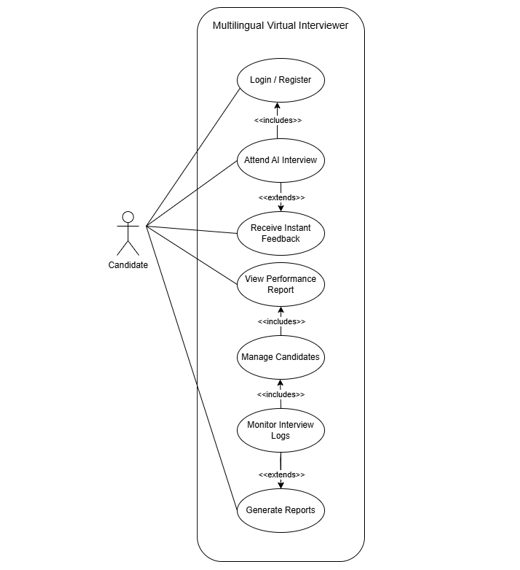
\includegraphics[width=0.8\textwidth]{AB.png}}
    \captionsetup{labelformat=empty}
    \caption{Figure \thefigure: Use Case Diagram}
\end{figure}
\vspace{10pt}

\noindent The Fig. 5.1 illustrates the use case diagram of the Multilingual Virtual Interviewer system for the Candidate actor. It represents the interaction between the candidate and the core functionalities of the system. The Login / Register function is the primary process that allows a candidate to securely create an account or access the platform. The Attend AI Interview use case is the central activity of the system and includes the Login / Register function, since authentication is required before participating in the interview.During or immediately after the interview, the system may provide instant results through the Receive Instant Feedback feature, which is shown as an extended function of the interview process. After the interview session is completed and evaluated, the candidate can access detailed results through the View Performance Report use case. This report presents the candidate’s performance, scoring, and evaluation insights generated by the system. Overall, the use case diagram clearly demonstrates how the candidate interacts with the system to register, participate in an AI-driven interview, receive feedback, and review performance in a structured and user-friendly manner.

\vspace{1cm}
% SUB-SUBSECTION 5.1.1: Use Case Document
\subsubsection{Use Case Document}
\vspace{10pt}

\begin{table}[H]
\centering
\renewcommand{\thetable}{5.1.1}

\small

\renewcommand{\arraystretch}{1.2}
\setlength{\tabcolsep}{4pt}

\begin{tabular}{|p{2.5cm}|p{5.2cm}|p{5.2cm}|}
\hline
\textbf{Actor} & \textbf{Description} & \textbf{Use Cases} \\
\hline

\textbf{Candidate} &
The Candidate is the primary actor who interacts with the Multilingual Virtual Interviewer system to participate in AI-driven interviews. The candidate registers on the platform, attends the interview session, responds to questions, and receives performance evaluation and feedback. &
- Login / Register \newline
- Attend AI Interview \newline
- Answer Questions (Voice/Text) \newline
- Receive Instant Feedback \newline
- View Performance Report \newline
- View Scores and Evaluation \newline
- Review Strengths and Weaknesses \newline
- Download / Save Report \\
\hline

\textbf{AI Interview System} &
The AI Interview System acts as the automated processing unit that manages the interview workflow. It handles authentication, question delivery, multilingual communication, response analysis, scoring, and report generation. &
- Authenticate Candidate \newline
- Conduct Interview Session \newline
- Deliver Questions \newline
- Process Voice/Text Responses \newline
- Perform Language Translation \newline
- Analyze Responses Using AI \newline
- Generate Scores and Feedback \newline
- Create Performance Report \newline
- Store Interview Data \\
\hline

\end{tabular}

\normalsize

\caption{Use Case Document}
\end{table}

\newpage
% SUB-SUBSECTION 5.1.2: Use Case Analysis
\subsubsection{Use Case Analysis}
\begin{enumerate}

    \item { Login / Register }  
    \begin{itemize}
The candidate creates a new account or logs into the system using valid credentials. During registration, the candidate provides necessary details such as name, email, and password. Secure authentication mechanisms verify the identity and grant access to the platform. Successful login enables the candidate to use all interview-related features.
    \end{itemize}

    \item { Attend AI Interview }  
    \begin{itemize}
After authentication, the candidate participates in the AI-driven interview session. The system presents questions in a structured sequence, which the candidate answers through voice or text input. The interview simulates a real interview environment and supports multilingual interaction to ensure accessibility for users from different language backgrounds.
    \end{itemize}

    \item { Response Submission }  
    \begin{itemize}
During the interview, the candidate submits responses to each question. The system captures spoken answers using speech-to-text technology or accepts typed responses. These responses are processed in real time for further analysis, ensuring accurate recording of the candidate’s input.
    \end{itemize}

    \item { Receive Instant Feedback }  
    \begin{itemize}
Upon completion of the interview or individual questions, the system may provide immediate feedback to the candidate. This feedback can include performance indicators such as correctness, communication clarity, confidence level, and language usage, helping the candidate understand their strengths and areas for improvement.
    \end{itemize}

    \item { View Performance Report }  
    \begin{itemize}
After the interview session is fully processed, the candidate can access a detailed performance report. The report contains scores, evaluation results, feedback summaries, and recommendations for improvement. Candidates may also review their performance history or download the report for future reference.
    \end{itemize}

\end{enumerate}

\newpage

% SUBSECTION 5.2: CLASS DIAGRAM
\subsection{Class Diagram}
\vspace{10pt}

\noindent The class diagram represents the object-oriented design of the Multilingual Virtual Interviewer system, illustrating how various components collaborate to conduct intelligent, AI-driven interview sessions. The Candidate interacts with the system through the User Interface, which serves as the primary communication layer and manages functions such as user authentication, profile access, interview participation, language selection, and report viewing. The Interview Module governs the entire interview lifecycle by initializing sessions, presenting context-appropriate questions, managing timing constraints, and collecting candidate responses in either voice or text format. These responses are forwarded to the Language Processing Module, which performs speech-to-text conversion, translation, and semantic analysis to enable multilingual interaction.The processed input is then evaluated by the AI Evaluation Module, which applies predefined assessment criteria and intelligent scoring algorithms to analyze communication skills, content relevance, and overall performance. The Administration Module allows authorized administrators to monitor system usage, manage users, configure question banks, and generate analytical reports. All system data is handled through a centralized Data Management component that interacts with underlying storage systems, including the User Database, Question Repository, Evaluation Records, and Analytics Data. This structured design ensures modularity, scalability, maintainability, and efficient coordination among system components while supporting real-time feedback and comprehensive performance analysis for both candidates and administrators.
\newpage
\begin{figure}[h]
    \centering
    \setlength{\fboxrule}{1pt} % Border thickness
    \setlength{\fboxsep}{0pt} % Space between image and border
    \renewcommand{\thefigure}{5.2} % Manual figure number
    \fbox{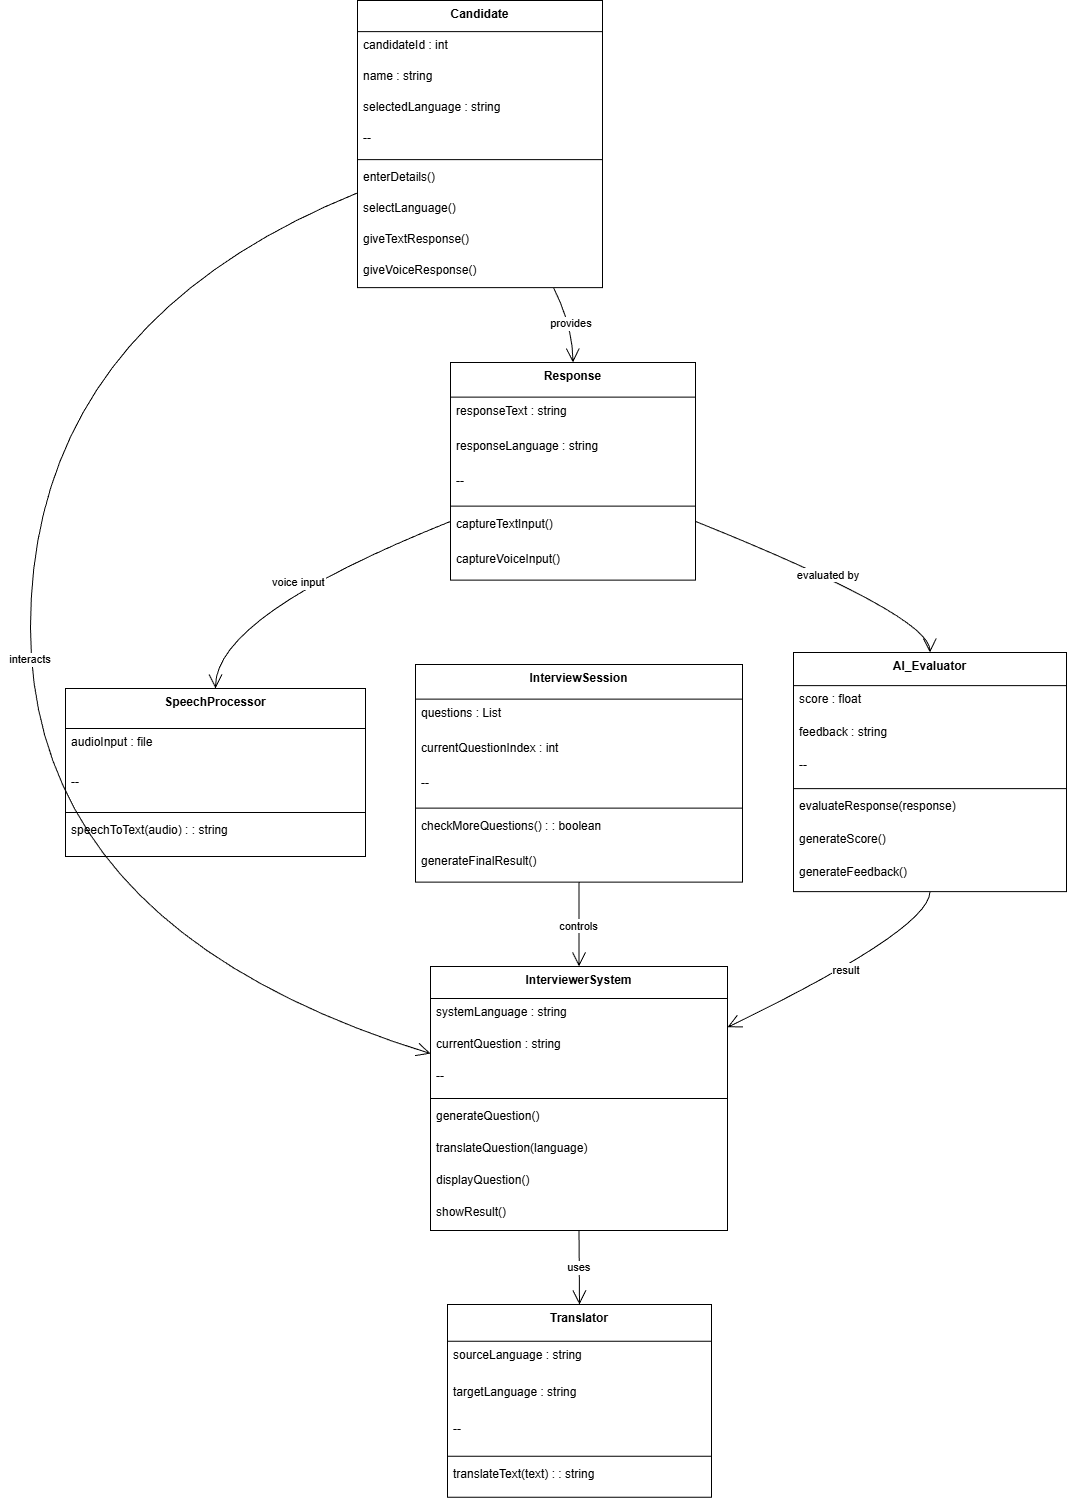
\includegraphics[width=0.7\textwidth]{Class Dig.png}}
    \captionsetup{labelformat=empty} % Remove default "Figure X.Y:"
    \caption{Figure \thefigure: Class Diagram}
\end{figure}

\newpage
% SUBSECTION 5.3: ACTIVITY DIAGRAM
\subsection{Activity Diagram}

\vspace{10pt}

\noindent The activity diagram shows the complete working flow of the Multilingual Virtual Interviewer system from the candidate’s perspective. The process begins when the candidate accesses the platform and logs in or registers using valid credentials. After successful authentication, the system displays the interview dashboard and allows the candidate to start the AI interview session. Once the interview begins, the system presents questions sequentially, and the candidate responds using voice or text input.The system captures the responses in real time and processes them using speech-to-text conversion, translation, and language analysis to support multilingual interaction. Each response is evaluated by the AI module for correctness, clarity, sentiment, and confidence. Based on the candidate’s performance, the system may adjust the difficulty or type of subsequent questions to simulate an adaptive interview process.After all questions are completed, the system analyzes the overall performance and generates scores along with feedback. Instant feedback may be displayed to the candidate, followed by a detailed performance report containing evaluation results and improvement suggestions. The candidate can view or download the report, after which the session ends or the user logs out. Overall, the activity diagram illustrates the step-by-step workflow of conducting an intelligent, automated interview from login to final evaluation.

\newpage

\begin{figure}[H] % Changed from [h] to [H] to force placement
    \centering
    \renewcommand{\thefigure}{5.3} % Manual figure number
    \fbox{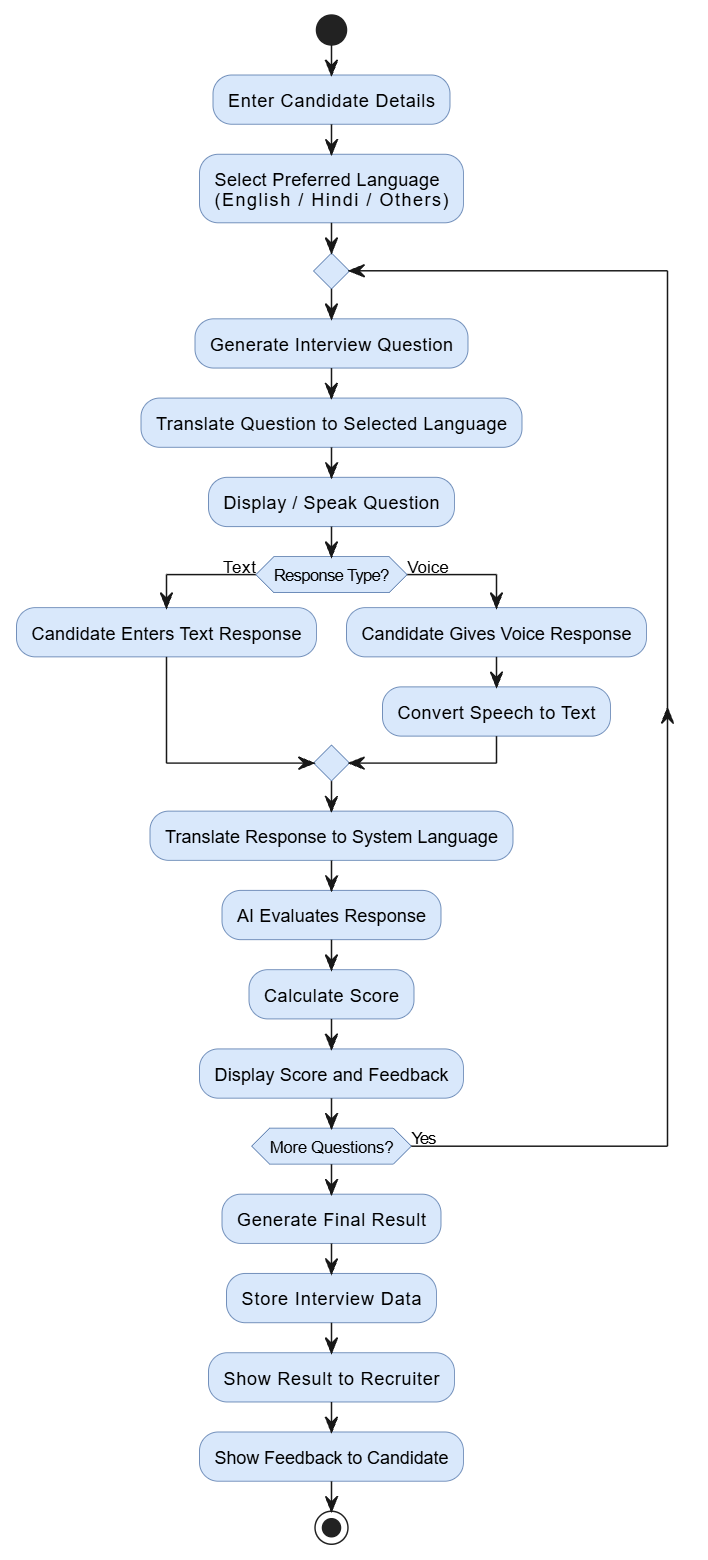
\includegraphics[width=1.5\textwidth, height=0.9\textheight, keepaspectratio]{ACTIVITY DIG.png}} % Added height and keepaspectratio
    \captionsetup{labelformat=empty} % Remove default "Figure X.Y:"
    \caption{Figure \thefigure: Activity Diagram}
    \label{fig:Activity}
\end{figure}

\newpage

% SUBSECTION 5.4: SEQUENCE DIAGRAM
\subsection{Sequence Diagram}

\vspace{10pt}

\noindent The sequence diagram illustrates the interaction between the Candidate, User Interface, Authentication Module, Interview Module, Language Processing Module, AI Evaluation Module, and Report Generator within the Multilingual Virtual Interviewer system. The process begins when the candidate accesses the platform and submits login or registration details through the user interface. The authentication module verifies the credentials and grants access to the interview dashboard upon successful validation.When the candidate starts the interview, the interview module presents questions sequentially through the interface. The candidate submits responses using voice or text input, which are forwarded to the language processing module for speech-to-text conversion, translation, and linguistic analysis to support multilingual communication. The processed responses are then passed to the AI evaluation module, which analyzes them for correctness, clarity, sentiment, and confidence.Based on this analysis, the system records scores and may adjust subsequent questions to maintain an adaptive interview flow. After all responses are collected, the evaluation results are sent to the report generator, which compiles a comprehensive performance report. The final report is displayed to the candidate through the user interface and stored in the system database for future access. The sequence concludes when the candidate views the results and logs out, completing the interaction cycle.

\begin{figure}[h]
    \centering
    \setlength{\fboxrule}{1pt} % Border thickness
    \setlength{\fboxsep}{0pt} % Space between image and border
    \renewcommand{\thefigure}{5.4} % Manual figure number
    \fbox{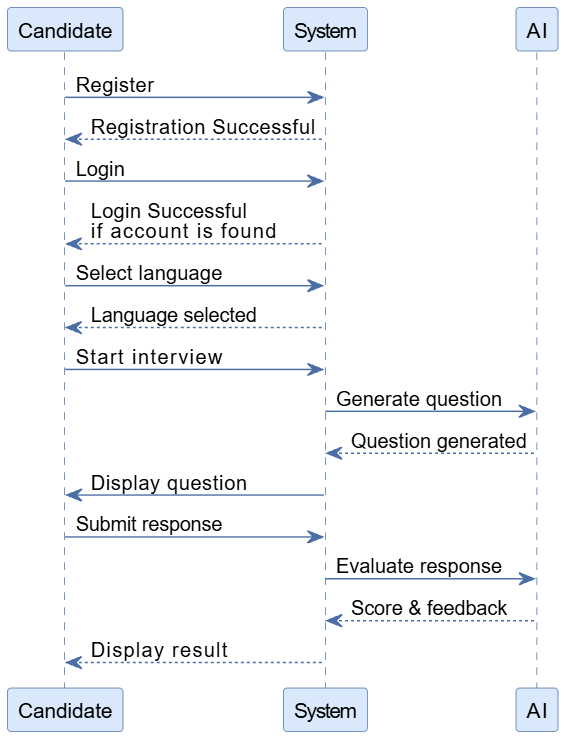
\includegraphics[width=0.9\textwidth]{sequence.png}}
    \captionsetup{labelformat=empty} % Remove default "Figure X.Y:"
    \caption{Figure \thefigure: Sequence Diagram}
\end{figure}



\end{document}